
%----------------------------------------------------------------------------------------
%	CHAP Analysis
%----------------------------------------------------------------------------------------

\chapterimage{blue-chapter-head_4-reduced.pdf} % Chapter heading image

\chapter{Analyses}\label{chap:Analyses}


\section{The MetaR Analysis Root Node}
MetaR analyses are represented with an Analysis AST Root node. An analysis often imports one or more tables, performs data transformations and writes a table or generates some plots. 
You can create as many Analysis root nodes as needed in a model. You create an analysis by right-clicking on a model and selecting \menu{New > o.c.metar.tables > Analysis}. Analysis can exist as direct child of a model, and for this reason is called a root node. Figure~\ref{fig:NewAnalysis} presents a new Analysis root node. 

\begin{SCfigure}
  \centering
  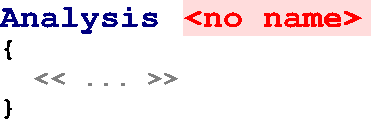
\includegraphics[width=\figWidthTiny]{figures/NewAnalysis.pdf}
\caption[New MetaR Analysis Root Node.]{\textbf{New MetaR Analysis Root Node.} This figure presents a freshly created MetaR analysis root node. You can press \keys{\return} over the \mpsplaceholder{} to add Statement nodes to the analysis. Use auto-completion to discover which types of statements are available. }
\label{fig:NewAnalysis}
\end{SCfigure}

\paragraph{name}
Each analysis has a name. You should name the analysis after creating it. The name you enter will be shown in the Project Tab after the 
\includegraphics[height={2ex}]{figures/analysis.png} icon.

\paragraph{statements}
An analysis contains a list of statements. You can enter new statements by typing between the curly brackets \texttt{\{} \texttt{\}}. 

To enter a specific statement, you can type the \texttt{alias} of the statement (for instance \texttt{import table}). When you have typed a complete alias, the node will be inserted in place of the alias. Note that there is no actual indication that the text you are typing matches a valid alias. You need to finish typing the full alias before the node is substituted for the alias. The text you type will remain red until the substitution occurs even if the text is matching a valid alias. See Figure~\ref{fig:TypingStatementAliases}.

\noindent The following sections describe the kinds of statements offered by the MetaR \texttt{org\allowbreak.campagnelab\allowbreak.MetaR\allowbreak.tables} language. The simplest way to learn which statements are supported by the release of MetaR that you are using is to use auto-completion. Figure~\ref{fig:AutoCompletionForStatements} provides a snapshot of the auto-completion menu when looking for statements to insert in the Analysis statement list. 
\begin{figure}[h!tbp]
  \centering
  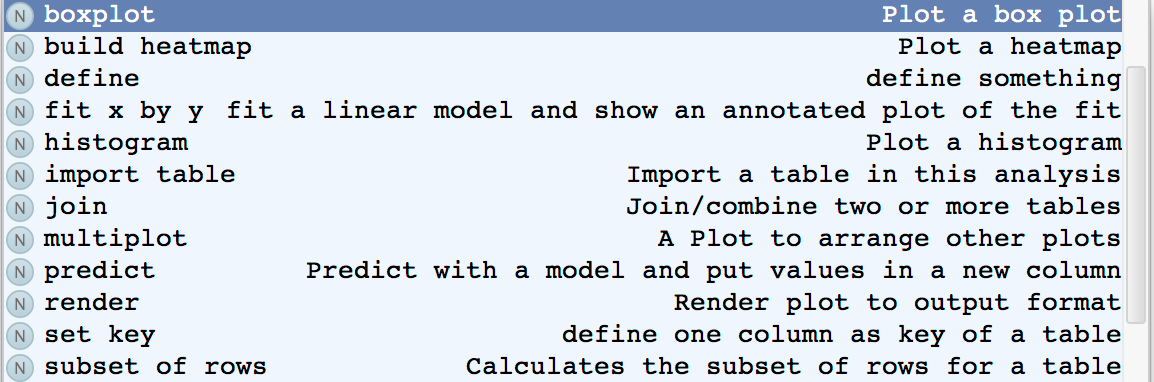
\includegraphics[width=\figWidthWide]{figures/StatementAuto-completion.png}
\caption[Auto-completion Dialog for Statements.]{\textbf{Auto-completion Dialog for Statements.} This dialog is obtained by placing the cursor where a Statement is valid, and pressing \keys{\ctrl+\space}.}
\label{fig:AutoCompletionForStatements}
\end{figure}



\begin{figure}[h!tbp]
  \centering
  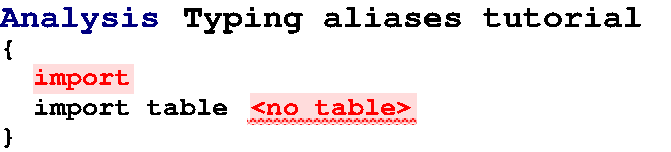
\includegraphics[width=\figWidthNarrow]{figures/AnalysisTypingAliases.pdf}
\caption[Typing Statement Aliases.]{\textbf{Typing Statement Aliases.} The user has typed ``import'' on the third line. This text is a prefix of the import table statement, but is shown in red because the alias is not yet complete. The fourth line shows the import statement which is substituted to the text when the user has just finished typing ``import table'', the complete alias of the statement. Note that pressing \keys{\return} immediately after import will create the node if the prefix ``import'' matches a single type of node in the languages imported in this model.}
\label{fig:TypingStatementAliases}
\end{figure}

\section{Working with Tables}

\subsection{Import Table}
The \texttt{import table} statement makes it possible to import a table, defined in the model, into the analysis. The columns of the imported table will become visible to the statements that follow the import. You can create an import table statement by typing the alias \texttt{import table} on an empty line of Analysis. Once you have bound the reference to a table, the import statement will look like this: 
\includegraphics[height=2ex]{figures/SomeDataImportTable.pdf}. The name in green is the name of the table the statement imports. See Section\ref{sec:CreateATable} to learn how to create a Table Root node.
\paragraph{table}

The table attribute is a reference to an AST root node. You can set this reference by typing the name of the table you wish to import, or by using auto-completion \keys{\ctrl+\space} to locate the table AST root node.

\subsection{Write Table}
MetaR analyses can create new tables. You can write the data in these tables to a file using the \texttt{write} statement (see Figure~\ref{fig:NewWriteTableStatement} for a new write statement). The write statement has two attributes: table and filename.
\begin{SCfigure}
  \centering
  
\includegraphics[width=\figWidthNarrow]{figures/NewWriteStatement.pdf}
\caption[New Write Statement	.]{\textbf{New Write Statement.} Use this statement to write the content of a table to a file.}
\label{fig:NewWriteTableStatement}
\end{SCfigure}


\paragraph{table}
This reference should be set to the table that you want to write to a file.
\paragraph{output}
The output should be set to a filename where you want the data contained in the table to be written. Notice that output has a button to let you select the output filename.

\subsection{Identify a Set of Columns}\label{subsec:KeySelectionDescription}
Several types of statements require the user to select one or more columns of a table. MetaR provides several ways to select a set of columns. 
\begin{itemize}
  \item You can use the \texttt{columns} node to identify a set of columns. 
  \item You can use the \texttt{group} node to name a single group, and identify all columns annotated with this group.
  \item You can use the \texttt{groups} node to name a set of groups, and identify all columns annotated with any of these groups.
\end{itemize}

\noindent{}Each strategy identifies a set of columns, which may contain one or more columns.

\section{Subset Rows}\index{Subset rows}\index{Filter rows}
You can use this statement (alias \texttt{subset rows}) to filter a table and produce a new table with a subset of the rows of the input table. Figure~\ref{fig:NewSubsetRows} shows a new \texttt{subset rows} statement.

\begin{SCfigure}
  \centering
  
\includegraphics[width=\figWidthNarrow]{figures/NewSubsetRowsStatement.pdf}
\caption[New Subset Rows Statement.]{\textbf{New Subset Rows Statement.} Use this statement to filter the rows of a table.}
\label{fig:NewSubsetRows}
\end{SCfigure}

\paragraph{table}
The input table reference must be set to a table. The table must be either imported or produced by another statement.
\paragraph{filter}
The filter determines which rows are kept. Use auto-completion to select one of the alternatives:
\begin{enumerate}
	\item \texttt{when true:} will keep a row when the boolean expression following when \texttt{true:} evaluates to  \texttt{true}.
	\item \texttt{with IDS} will keep a row when the value of the column marked with group \texttt{ID} exists in the list provided as an argument. See the \texttt{define} statement to create a list of IDs. 
\end{enumerate}

\paragraph{subset}
The output table is called subset by default. Feel free to rename this table to better match the data in it.

\subsection{Example}
Figure~\ref{fig:ExampleSubsetRows} presents examples of subset row statements. 

\begin{figure}[h!tbp]
  \centering
  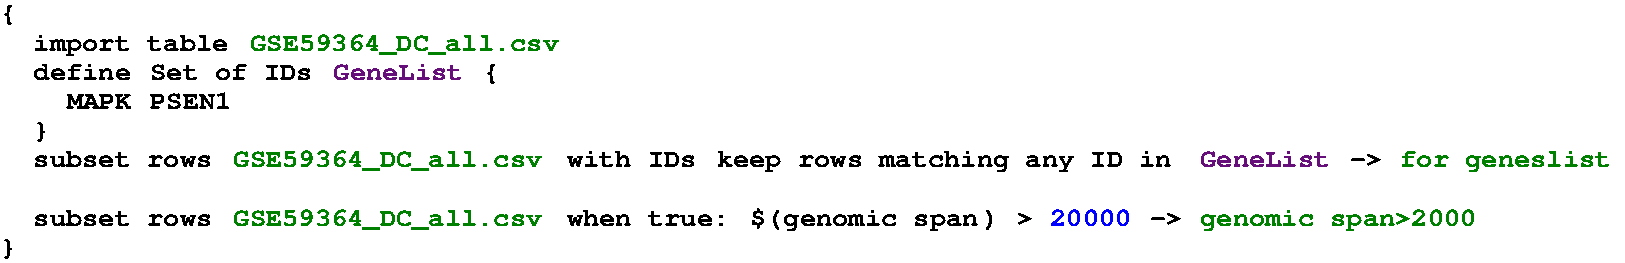
\includegraphics[width=\figWidthWide]{figures/ExampleSubsetRows.pdf}
\caption[Subset Rows Examples.]{\textbf{Subset Rows Examples.} This figure illustrates the two alternatives available for filtering rows: by expression (with \texttt{when true:}, or with a set of ID values).}
\label{fig:ExampleSubsetRows}
\end{figure}

\subsection{Boolean Expressions}
One form of the subset rows statement accepts a boolean expression to determine which rows to keep. Boolean expression have one of two values: true or false, and can be constructed by comparing values with an operator. The following operators are supported by MetaR:
\begin{itemize}
 \item \textbf{\$(} column \textbf{)} The value operator evaluates to the value of the column in the row currently considered.
	\item expr1 \textbf{==} expr2 true when expr1 evaluates to the same value as expr2.
	\item expr1 \textbf{!=} expr2 true when expr1 does not evaluate to the same value as expr2.
	\item expr1 \textbf{|} expr2 true when expr1 is true or expr2 is true (boolean or. either one of expr1 or expr2 needs to be true for the result to be true).
    \item expr1 \textbf{\&} expr2 true when expr1 is true and expr2 is true (boolean and, both expre1 and epr2 must be true for the result to be true).
    \item expr1 \textbf{<} expr2 true when expr1 evaluates to a value less than expr2.  
    \item expr1 \textbf{>} expr2 true when expr1 evaluates to a value greater than expr2.  
   \item expr1 \textbf{<=} expr2 true when expr1 evaluates to a value less or equal than expr2.  
    \item expr1 \textbf{>=} expr2 true when expr1 evaluates to a value greater or equal than expr2.  
\end{itemize}

\begin{remark}
MetaR infers the type of the expressions that you enter and will report type errors if the value of some values are not compatible with the test that your perform.
\end{remark}

\section{Join Tables}\index{Join Tables}
When you perform data analysis, you often need to combine data from different tables into one. This operation is called table joining. MetaR provides a powerful \texttt{join} statement that helps join an arbitrary number of tables. The alias of the statement is \texttt{join}. Figure~\ref{fig:NewJoinStatement} presents a newly created \texttt{join} statement. Join has three attributes: input tables, by and output table.

\begin{SCfigure}
  \centering
  
\includegraphics[width=\figWidthNarrow]{figures/NewJoinStatement.pdf}
\caption[New Join Statement.]{\textbf{New Join Statement.} Use this statement to join two or more tables into one.}
\label{fig:NewJoinStatement}
\end{SCfigure}

\paragraph{input tables}
Use this attribute to enter references to tables you need to join. You can press \keys{\return} with the cursor inside the parentheses to create references to additional input tables (either imported or created in the analysis up to that point).
\paragraph{by}
Use the by attribute to specify how to join the input tables. Joining tables requires knowing which rows of the input tables go together. This is done by identifying a set of columns whose values must match across rows of the input tables that go together. See Section~\ref{subsec:KeySelectionDescription} to learn how to select groups of columns in MetaR. You can select one of the following joining strategies as value of the by attribute:

\begin{itemize}
	\item \textbf{by columns:} The same column name must be defined in all the input tables.
	\item \textbf{by group:} If each table has exactly one column annotated with this group, the names of the columns do not need to be the same. Otherwise, if more than one columns is in the group, their names must match across all the tables. 
	\item \textbf{by groups:} Similar to group, but with any (>=1) number of groups. Press \keys{\return} to insert new group references.
\end{itemize}
 The group by columns are used to calculate a list of values. When rows of the input tables have the same group by values, they are joined in a single row, and the result put in the destination table. 

\begin{remark}
The join statement will create new columns if the input tables have columns with the same name. In this case the shared columns are renamed ``colname.TableName''. Place the cursor on result and look at the column preview in the inspector to see which column names are generated by a given join statement.
\end{remark}

\paragraph{result}
The output table is called Results by default. Feel free to rename this table to match the content of the destination table. Open the \inspectorTabIcon{} to see which columns will result from the join. Notice that the column groups are transfered to the columns of the output table.


\subsection{Example Join}\index{Example}\index{Join}
Figure~\ref{fig:ExampleJoinStatement} presents an example of join statement. The statement joins two tables and creates the Result table. If you open the \inspectorTabIcon{}, you will see a preview of the columns for the result table (shown in Figure~\ref{fig:ColumnPreviewExample}). 
\begin{SCfigure}
  \centering
  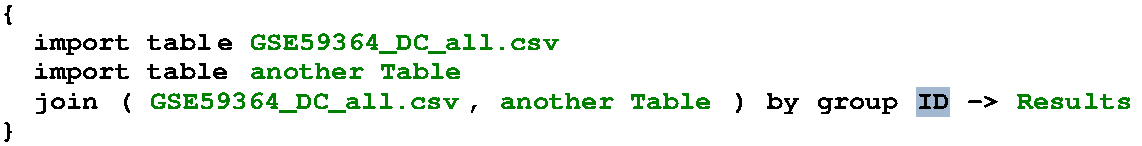
\includegraphics[width=\figWidthNarrow]{figures/ExampleJoin.pdf}
\caption[Example of Join Statement.]{\textbf{Example of Join Statement.}}
\label{fig:ExampleJoinStatement}
\end{SCfigure}


\begin{figure}[h!tbp]
  \centering
  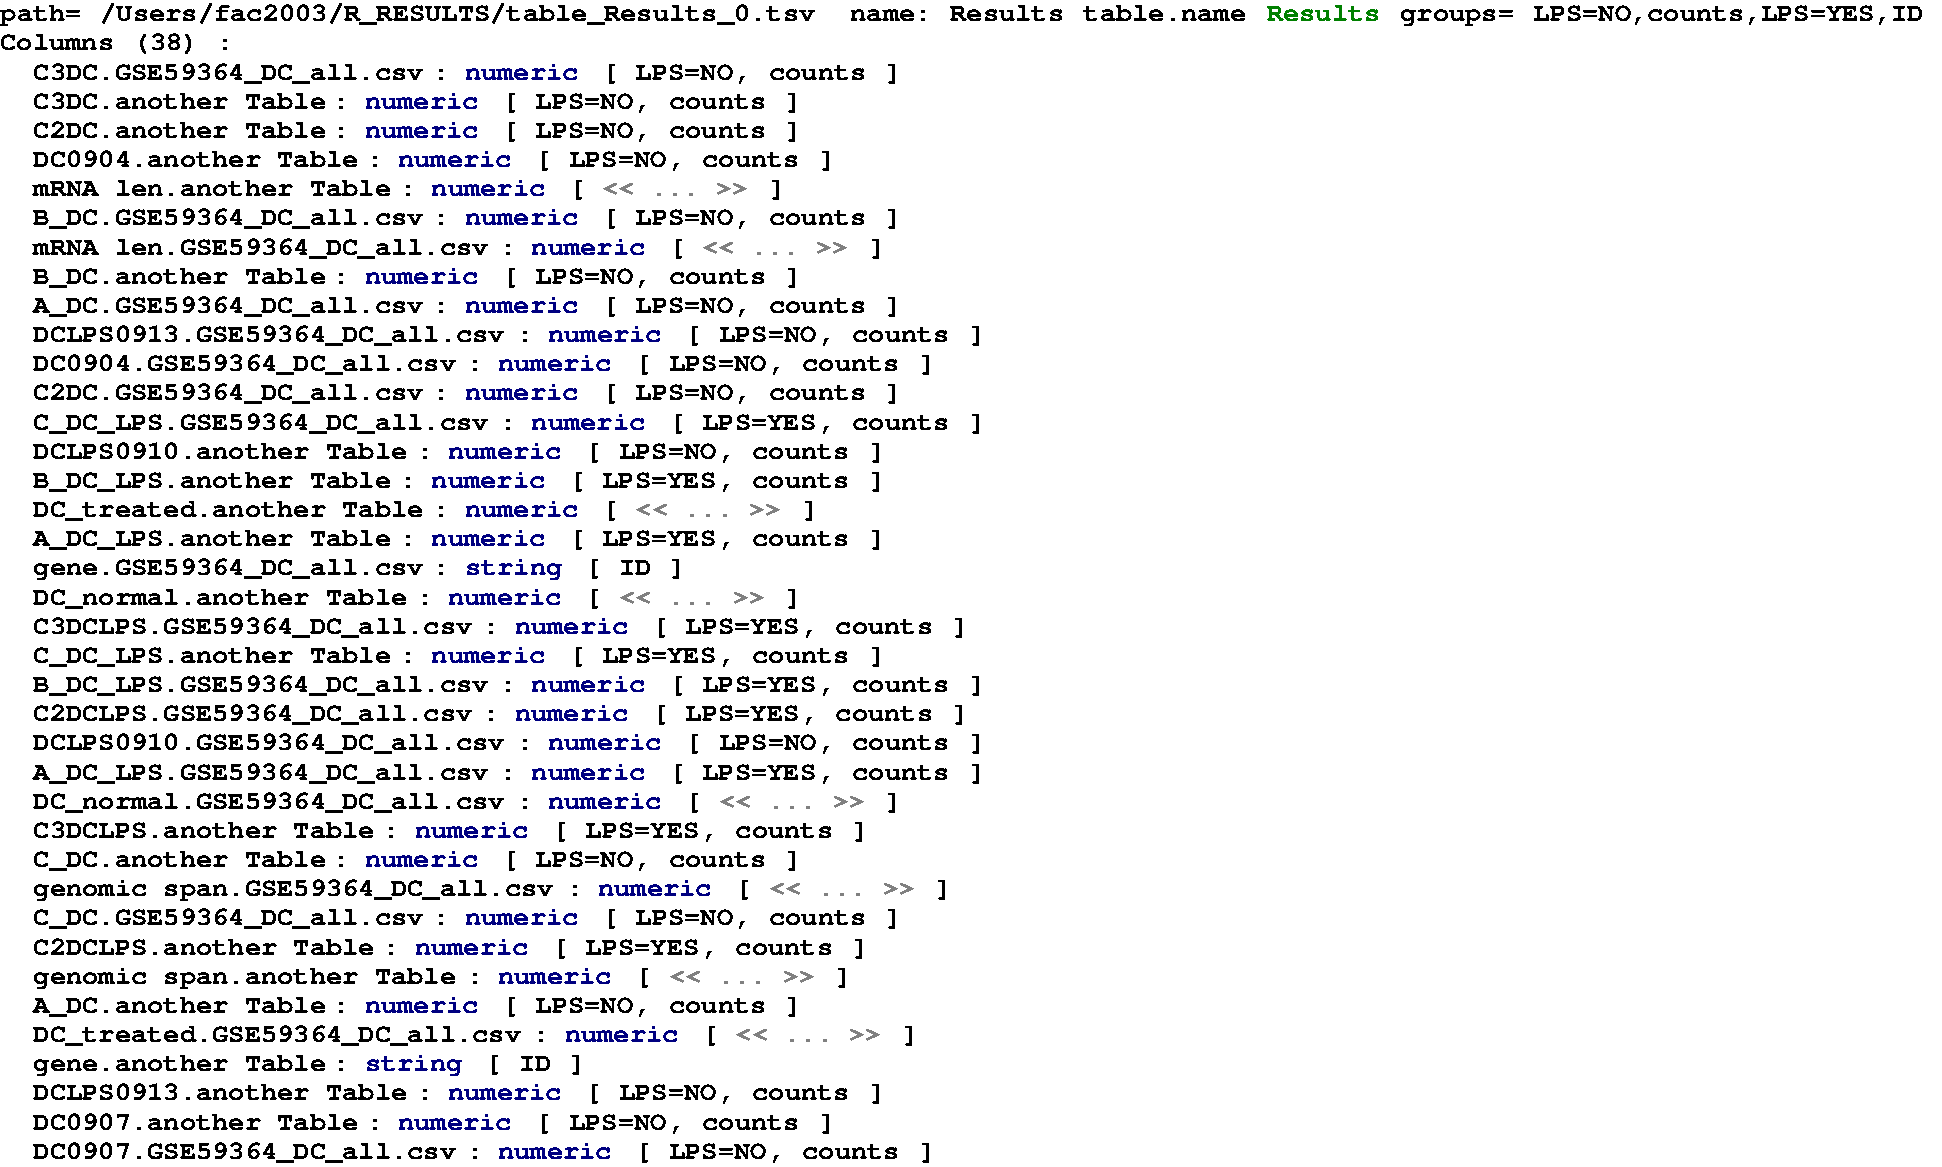
\includegraphics[width=\figWidthWide]{figures/ExampleJoinColumnPreview.pdf}
\caption[Column Preview for Result Table.]{\textbf{Column Preview for Result Table.} Notice that all these columns were shared across the input tables because their name follows the pattern ``colName.tableName''.}
\label{fig:ColumnPreviewExample}
\end{figure}


\section{Plotting Data}
MetaR provides simple plotting capabilities\footnote{These capabilities are simple, but can be extended very easily by adding new statements to draw other types of visualization. This is a key advantage of using Language Workbench technology.}. The following types of plots are currently supported: 
\begin{itemize}
  \item boxplot alias \texttt{boxplot}
  \item histogram alias \texttt{histogram}
  \item scatterplot: alias \texttt{fit}
  \item heatmap, alias \texttt{heatmap}
  \item multiplot alias \texttt{multiplot}, makes it possible to organize other plots in a matrix of n columns by n rows.
\end{itemize}
Each type of plot statement will create a plot, identified with the 
\includegraphics[height=2ex]{figures/plot.png} icon when you are trying to auto-complete a reference to a plot. Plot names are also colored with the same dark blue as the icon.

\subsection{boxplot}\index{BoxPlot}
Figure~\ref{fig:NewBoxPlot} presents a new boxplot statement.

\begin{SCfigure}
  \centering
  
\includegraphics[width=\figWidthNarrow]{figures/NewBoxplot.pdf}
\caption[New Boxplot Statement.]{\textbf{New Boxplot Statement.}}
\label{fig:NewBoxPlot}
\end{SCfigure}

\paragraph{columns}
Indicate one or more columns to plot. The values of the columns will be plotted as individual boxplots in the same graph. Press \keys{\enter} to define more than one column. Use auto-completion to locate individual columns from the imported tables, or the tables created by prior statements. 

\paragraph{plot}
The attribute after \texttt{->} is a plot. Enter a name for the boxplot here. Plot names are colored blue to make them easier to recognize.

\paragraph{style}
Different kind of plots accept different types of styles. The boxplot accepts a \texttt{Color\allowbreak{}Plot\allowbreak{}Style}. You can create this node in the model and bind the boxplot statement to it to customize the colors that will be used to draw this boxplot. 


\subsection{histogram}\index{Histogram}
Use this statement to plot a histogram of the values of one column.
\paragraph{column}
Indicate one column to plot a histogram for. Use auto-completion to locate the column from the imported tables, or the tables created by prior statements. 

\paragraph{plot}
The attribute after \texttt{->} is a plot. Enter a name for the histogram here. Plot names are colored blue to make them easier to recognize.

\paragraph{style}
Different kind of plots accept different types of styles. The histogram accepts a \texttt{Color\allowbreak{}Plot\allowbreak{}Style}. You can create this node in the model and bind the histogram statement to it to customize the colors that will be used to draw this plot. 



\subsection{fit x by y}
Use this statement (alias \texttt{fit}) to plot a scatter plot of x (one column) vs y (another column). A fit is performed, and the R2 adjusted, and P-value corresponding to the linear regression is shown on the plot. Figure~\ref{fig:NewFitXByY} presents a new \texttt{fit} statement.

\begin{figure}[h!tbp]
  \centering
  
\includegraphics[width=\figWidthWide]{figures/NewFitXByY.pdf}
\caption[New Fit X by Y.]{\textbf{New Fit X by Y.}}
\label{fig:NewFitXByY}
\end{figure}

\paragraph{x, y}
Indicate which columns should be plotted. Use auto-completion to locate the x and y columns from the imported tables, or the tables created by prior statements. 

\paragraph{plot}
The attribute after \texttt{->} is a plot. Enter a name for the scatterplot here. Plot names are colored blue to make them easier to recognize.

\paragraph{style}
Different kind of plots accept different types of styles. The fit statement accepts a \texttt{Scatter\allowbreak{}Plot\allowbreak{}Style}. You can create this node in the model and bind the fit statement to it to customize the title, axes and range of data in the scatterplot. Figure~\ref{fig:NewScatterPlotStyle} shows the attributes of the \texttt{ScatterPlotStyle} node.

\begin{remark}
Styles will refactored in a future version of MetaR to improve their flexibility and remove redundant style definitions. This documentation does not describe styles in detail for the moment, and will be updated to describe the new Style functionality. 
\end{remark}


\begin{SCfigure}
  \centering
  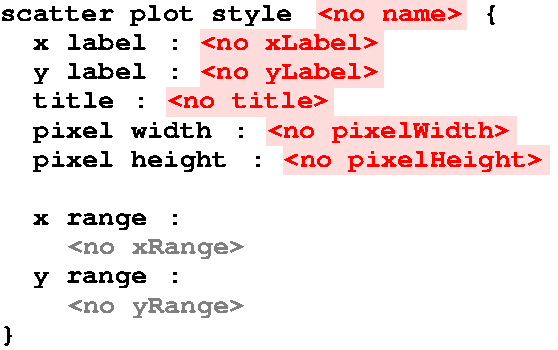
\includegraphics[width=\figWidthNarrow]{figures/NewScatterPlotStyle.pdf}
\caption[New Scatterplot Style.]{\textbf{New Scatterplot Style.}}
\label{fig:NewScatterPlotStyle}
\end{SCfigure}


\subsection{heatmap}\index{Heatmap}
Use this statement (\texttt{heatmap}) to construct a heatmap. Figure~\ref{fig:NewBuildHeatmap} presents a new \texttt{heatmap} statement.

\begin{figure}[h~tbp]
  \centering
  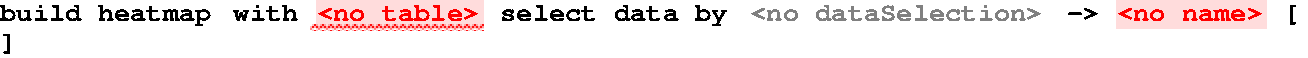
\includegraphics[width=\figWidthWide]{figures/NewBuildHeatmap.pdf}
\caption[New Heatmap.]{\textbf{New Build Heatmap.} Notice the intention ``Add Annotations'' attached to the statement. You can use this intention to further customize the heatmap.}
\label{fig:NewBuildHeatmap}
\end{figure}

\paragraph{table}
Specify the table that contains the data that will be used to draw the heatmap. Note that the table must meet certain conditions. An error message will be displayed if these conditions are not met:

\begin{itemize}
  \item Some columns of the table must be annotated with at least one group whose usage is ``heatmap''. Such columns are used to provide data values for the heatmap. If you don't have a heatmap usage, just create one and add it to the groups you would like to include on the heatmap.
  \item The columns of the table must be annotated with groups and group usages to make it possible for you to use these group usages to construct a legend.
\end{itemize}

\paragraph{select data by}
Use this attribute to customize the set of columns to plot on the heatmap. See Section~\ref{subsec:KeySelectionDescription} to learn how to select a set of columns.

\paragraph{plot}
The \texttt{<no name>} attribute listed after \texttt{->} makes it possible to name the plot that will hold the heatmap. Use any name you like. This name will be used to refer to the heatmap plot, for instance if you wish to assemble panels of different heatmaps into one figure.

\paragraph{annotations}
You can use the ``Attach Annotations'' intention (\intentionLightBulb) when the cursor is on top of \texttt{heatmap} to customize heatmap annotations. Figure~\ref{fig:BuildHeatmapWithAnnotations} shows a heatmap statement with annotations.

\begin{figure}[h!tbp]
  \centering
  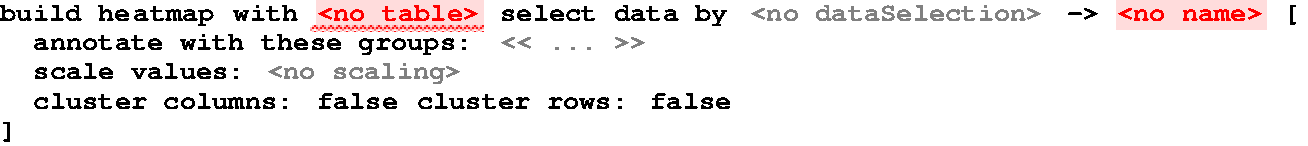
\includegraphics[width=\figWidthWide]{figures/NewBuildHeatmapWithAnnotations.pdf}
\caption[Heatmap With Annotations.]{\textbf{Build Heatmap With Annotations.} Annotations are shown after you have triggered the ``Add Annotations'' intention.}
\label{fig:BuildHeatmapWithAnnotations}
\end{figure}

\subparagraph{\textbf{annotate with these groups.}} You can use this attribute to select usage names that should be listed in the heatmap legend. Listing a group usage will annotate each column of data with the group that is associated to the usage.
\subparagraph{\textbf{scale values.}} You can choose to scale values by column or by row. Scaling will make differences easier to see by using colors more effectively.
\subparagraph{\textbf{cluster columns:}} You can choose to cluster by colors or by rows by changing the boolean values accordingly.

\subsubsection{Example}\index{Example}

\begin{figure}[h!tbp]
  \centering
  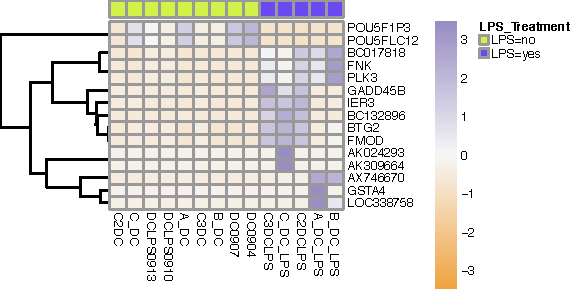
\includegraphics[width=\figWidthWide]{figures/heatmap_Example.pdf}
\caption[Example of Heatmap Plot.]{\textbf{Example of Heatmap Plot.} This heatmap has been customized with annotations. The \texttt{LPS\_Treatment} group usage is shown in the legend, with two groups: \texttt{LPS=yes} and \texttt{LPS=no}. The values plotted have been scaled by rows, and the rows clustered. Data are from \url{http://www.ncbi.nlm.nih.gov/geo/query/acc.cgi?acc=GSE59364}.}
\label{fig:ExampleHeatmapPlot}
\end{figure}

Figure~\ref{fig:ExampleHeatmapPlot} presents a heatmap constructed with the build heatmap statement, using annotations and row clustering. 

\subsection{multiplot}\index{Multiplot}
This statement (alias \texttt{multiplot}) makes it possible to assemble a plot as a matrix of $m$ x $n$ plots. This is convenient if you would like to create a figure from panels of individual plots. In addition, multiplot provides a preview of the multi-panel plot that you can turn on and off at the click of a button. Figure~\ref{fig:NewMultiplot} presents a new Multiplot.


\begin{figure}[h!tbp]
  \centering
  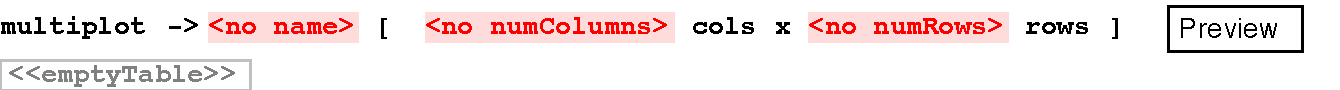
\includegraphics[width=\figWidthWide]{figures/NewMultiplot.pdf}
\caption[New Multiplot Statement.]{\textbf{New Multiplot Statement.} Click on the Preview/Hide Preview button to toggle the plot preview.}
\label{fig:NewMultiplot}
\end{figure}

\paragraph{plot}
The plot name is shown immediately after \texttt{->} (initially \texttt{<no name>}). Name the mutliplot to be able to refer to it from other statements (such as render to make a PDF from it).
\paragraph{$m$ cols x $n$ rows}
Define the number of columns and rows that you wish the multiplot to have. 
The product of $m$ and $n$ determines how many plot references must be filled in to construct the multiplot.

\paragraph{Preview/Hide Preview}
These buttons will make it possible to preview/ hide the preview for the multiplot. Note that a preview is only available after you have run the analysis. If you don't see the image being refreshed after running the script, remember to hide the preview and show it again to refresh.

\paragraph{plot references}
After you set the number of columns and rows, you need to link  $m$ x $n$ references to plots that you have already constructed. Do this in table attribute (shown as \texttt{<<emptyTable>>} initially).


\subsubsection{Multiplot Example}
Figure~\ref{fig:ExampleMultiplot} presents an example of multiplot.

\begin{figure}[h!tbp]
  \centering
  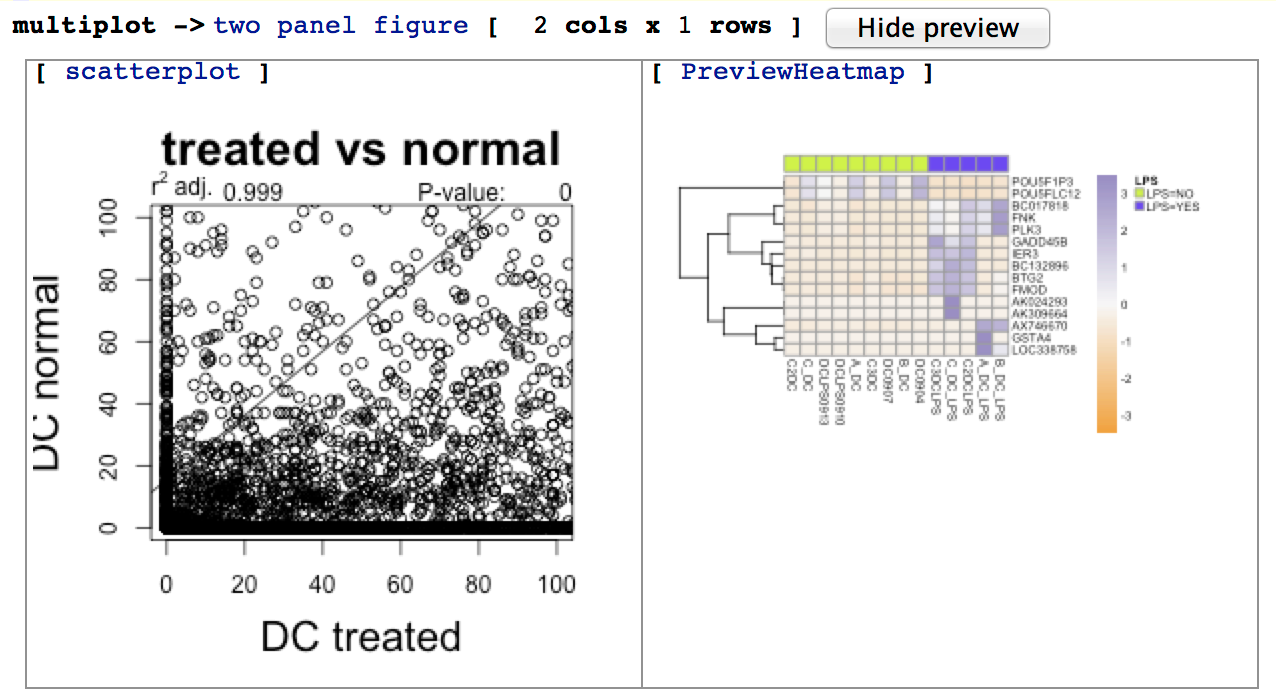
\includegraphics[width=\figWidthWide]{figures/MutliplotExample.png}
\caption[Example of Multiplot.]{\textbf{Example of Multiplot.} This example shows a multiplot composed of two columns and one row. In the preview,  a fit x by y plot is shown on the left, and a heatmap on the right. }
\label{fig:ExampleMultiplot}
\end{figure}

  
